\documentclass{thesis}
\usepackage{subfigure}
\usepackage{graphicx}
\usepackage{hyperref}
\usepackage{url}

\thesistitle{\bf Only Everything Lasts Forever}        
\author{Kyle McDonald}        
\degree{Master of Fine Arts}
\department{Electronic Arts}
\thadviser{Curtis Bahn}
\cothadviser{Michael Century}
\cocothadviser{Shawn Lawson}
\submitdate{May 2010\\(For Graduation May 2010)}
\copyrightyear{2010}
      
\begin{document} 
\titlepage
\tableofcontents
%\listoftables % required if there are tables
\listoffigures % required if there are figures

\specialhead{Acknowledgments}

This thesis represents the culmination of my time not only as an MFA student, but also as an undergraduate at RPI. Many of the ideas in this thesis would be difficult for me to conceptualize were it not for a few key undergraduate professors: Bram van Heuveln, Jim Fahey, Michael Zenzen, John M. Koller, David Gibson and Larry Kagan. As my vision for ``Only Everything Lasts Forever'' initially formed, I am indebted to Neil Rolnick, Curtis Bahn, and Shawn Lawson for defending it as a worthwhile endeavor. As it continued developing, I'm very grateful for my discussions with Caitlin Morris, Paolo Pedercini, Michael Century, Blair Neal, Mark Changizi, Daito Manabe, Pete Hellicar, Joel Gethin Lewis, Micah Silver, and Christian Karl Janssen. I feel very fortunate to have had conversations with some of the people who inspired this work, including Yasunao Tone, John F. Simon Jr., Dr. Martin Ruckert, Lars Eijssen, Rosa Menkman and Mats \"Oljare. Finally, I would like to thank my parents for supporting me in my enthusiasm despite my unending inability to explain what I'm working on at any given moment.

\specialhead{Abstract}

This thesis explores the definition of ``noise'' as ``non-contextual sound''. It defines ``context'' using examples from philosophy, science, and art, examining our ability as observers to misunderstand and misinterpret context. It presents the notion of an ``embedded context'', using examples from the sonic and visual arts. These examples reveal embedded contexts through empty work, glitches, enumeration, and unusual durations. The sound composition ``Only Everything Lasts Forever'' is presented, drawing on all these topics. This composition enumerates all the sounds we can distinguish as humans, as defined by the MP3 digital audio format. The historical and structural aspects of the MP3 format are discussed, along with a technique for enumerating the large space of MP3 in a way that exhibits variation on a human scale.

\chapter{Introduction}

Noise is an invention. Not only an invention, but a necessity: noise is misunderstanding. As long as there are observers, there will be noise---and without observers, there is no noise.

I define ``noise'' as ``non-contextual sound''. By ``context'' I am referring to the various relationships a system may have to itself and to other systems---relationships that are often misunderstood or misinterpreted. This definition is neither normative nor arbitrary; I use it in an attempt to describe my personal intuitions and general suspicions for how the word is used in practice.

This definition of noise follows a long tradition of theoretical, compositional and improvisational explorations of the term. A close definition to mine is ``that outside of a given representation'', given by Doug Van Nort\cite{Vannort06}. Similarly, Jean-Jacques Nattiez, says that musical meaning emerges ``when an object is placed in relationship to a horizon''\cite{nattiez_music_1990}. Or consider the numerous other perspectives on noise from signal processing and information theory, or composers like Luigi Russolo\cite{Russolo04}, John Cage\cite{Cage61} and Kim Cascone\cite{Cascone00}, or theorists like Jacques Attali\cite{Attali85}.

Rather than placing noise in the usual opposition to music, I will explore this definition directly. In Chapter 2, ``Understanding Context'', I will further define ``context'' using examples from philosophy, science, and art, focusing on our ability as observers to misunderstand and misinterpret it. In Chapter 3, ``Revealing Embedded Contexts'', I will introduce the notion of the ``embedded context'' of a medium, and discuss artwork focused on collaborating with and revealing these contexts. These examples reveal embedded contexts through empty work, glitches, enumeration, and unusual durations. Finally, in Chaper 4, ``Only Everything Lasts Forever'', I will discuss my work of the same title, informed by all the previously discussed topics.

``Only Everything Lasts Forever'' is a sound composition that enumerates all the sounds we can distinguish as humans as defined by the MP3 digital audio format. It lasts approximately $10^{452}$ years long, and is realized by custom software that regularly generates hour-long excerpts. It was composed with the intent of exhaustively contextualizing all distinguishable sounds, and exploring the conflation of a sound representation's limitations with our own perceptual limitations.

\chapter{Understanding Context}

\section{Metaphor, Coherence and Interdependence}

In ``Metaphors We Live By'', George Lakoff and Mark Jonhnson explore the thesis that our beliefs and actions are structured by a metaphorical ``web'' of understanding. The word ``context'' is itself rooted in a metaphor: the Latin ``contexere'' describes the ``joining together'' of weaving.\cite{douglas_harper_context_2010} In this paper, the word ``context'' refers to the intertwined relationships, rather than single foundation, supporting a system.\footnote{These relationships may be self-referential, as Douglas Hofstadter argues in the case of cognition.\cite{Hofstadter01} He describes not only cognition as analogical, but consciousness itself as fundamentally self-referential\cite{Hofstadter07}.} In accordance with metaphor as the foundation for understanding: when we have no context for a sound, we cannot conceptualize it so we call it noise.

In Western epistemology, context manifests itself as the coherence theory of truth\cite{Blackburn07}\cite{young_coherence_????}, where truth is identified by its coherence with other propositions. This theory stands in opposition to the correspondence\cite{david_correspondence_????} theory of truth, where truth is identified by correspondence to an external system. In accordance with coherence as the foundation for belief: when we have no context for a sound, we cannot identify its meaning, so we call it noise.

In Buddhist philosophy, context manifests itself in doctrine of \emph{pratityasamutpada}, or ``interdependent arising''\footnote{Cage uses the translation ``interpenetration'' to describe this concept.}, which accounts for the causal relationship between all things.\cite{Koller01} This is deeply tied to the notion of \emph{sunyata}, or ``emptiness'', which asserts that nothing has an inherent essence but exists only in relation to everything else---something that we frequently misunderstand\footnote{I use the word ``misunderstanding'' to refer to \emph{avidya}, also translated ``ignorance'' and ``delusion''.}. In accordance with the doctrines of interdependence and emptiness: all sounds have context, but we sometimes misunderstand that context and instead grasp for a non-existent inherent essence---we call it noise.

\section{A Signal Appears as Noise}

\begin{quote}
Take a photograph of your head inside a freezer. Upload this photo to the internet (like flickr). Tag the file with 241543903. The idea is that if you search for this cryptic tag, all the photos of heads in freezers will appear. I just did one.\cite{david_horvitz_flickr:_????-1}
\end{quote}

Sometimes the deeper context of apparent noise is later revealed. The above instructions were sent by David Horvitz to a mailing list in 2009.\cite{david_horvitz_for_2009} To a casual surfer, this unusual photo paired with a ``cryptic'' number would appear as noise. But once the context of Horvitz' instructions are revealed, the image and tag are no longer understood as noise. Alternatively, once enough photos are surveyed with the same theme and tag, the context becomes the set of images.\footnote{Also see ``MOOKDFJLAL''\cite{david_horvitz_flickr:_????}, where Horvitz instructs people to wear pillow cases over their heads.}

In the case of a tagged image, you might suspect a deeper context than the superficially obvious one. In computer security, apparently indecipherable noise can sometimes be reverse engineered to reveal a deeper context where none was originally even suspected---a context beyond intuition, but within the scope of computation. These ``side-channel attacks'' might consist of simply zooming in on a reflection of a screen at a distance to snoop on the displayed information,\cite{w._wayt_gibbs_hackers_2009} or recording the emitted RF radiation of a CRT monitor and amplifying it for display on another screen.\cite{erik_thiele_tempest_????} In a ``timing attack'', variations in a computer's sluggishness reveal the contents of its computation. The LED on a router may appear to blink at random, but they are sometimes driven directly by the data line---and can therefore be optically recorded and decoded.\footnote{Similar computer security techniques were infamously applied to daily life, as ``reality-cracking''\cite{francesco_vianello_reality_????}, by Fravia (Francesco Vianello)---a prominent software cracker who regularly published various technical details of his practice along with manifestos on cracking philosophy. He proposed: the same way line after line of assembly code may at first appear impenetrable and unrelated to the program it represents, the chaos of daily life may seem irrelevant to our belief systems and practices and those of others around us. But they are related, and it only takes time to understand the ``concealed truths''. Fravia was particularly focused on ``seeing through'' consumerism, but was interested in everything---including body language, food additives, war propaganda, telemarketing, and bottled water.}

An initial encounter with 241543903 or the data behind side-channel attacks are examples of ``misunderstood context'': hearing sounds as ``noise'' because their context is not initially understood, or the understood context is only superficial\footnote{Awareness of one's reliance upon others is a more superficial context, while understanding of precisely who and how one is reliant on others is a deeper context. Attended sound has the superficial context of simply being attended, but may also contain emotional, musicological, natural, or other deeper contexts.}.

\section{Noise Appears as a Signal}

An observer may filter noise until it gains a perceptually relevant context. This is a kind of ``misinterpreted context''. Humans have an especially strong bias for anthropomorphization: astronomical features like the face on Mars\cite{brian_dunning_facemars_2008} and the CfA2 Great Wall ``stick man''\cite{valrie_de_lapparent_slice_1986}, religious figures like Jesus, Mary and Saraswati in stains and foods\cite{_iron_????}\footnote{Dan Paluska satirizes these sightings with his ``Holy Toaster''\cite{dan_paluska_holy_2005}: an art object and commercially available toaster insert that burns the face of Jesus onto every piece of toast inserted.} and Ganesha in mathematical visualizations\cite{melinda_green_buddhabrot_1993}, or the ghosts of the Ganzfeld effect and electronic voice phenomena\footnote{In ``Ghosts in the Machine'' by Alan Dunning, Paul Woodrow, and Dr. Morley Hollenberg\cite{alan_dunning_paul_woodrow_and_morley_hollenberg_einsteins_2008}, a camera is placed inside a black box, with the image formed on the sensor amplified in software and automatic face detection applied. The computer then projects the image from the camera with a rectangle around any region identified as containing a ``face''.}. Even the iPod MP3 player was notoriously anthropomorphized when operating in shuffle mode.\cite{rachel_dodes_tuneshard_2004}

Gestalt theory describes some of these phenomena in terms of pattern recognition, covering cases of biologically informed context like the Kanizsa triangle illusion\cite{alexander_bogomolny_kanizsa_????} and experientially acquired context as in the case of the dalmatian illusion\cite{michael_bach_dalmatian_2002}. Other systems are more dependent on transformation through intellectual reflection: the Bible Code\footnote{Originally ``Equidistant Letter Sequences in the Book of Genesis''\cite{doron_witztum_eliyahu_rips_and_yoav_rosenberg_equidistant_1994}.} and Jonathan Feinberg's ``Haiku Finder'', the Voynich manuscript\cite{robin_mckie_secret_2004}, the Golden Ratio\cite{Doczi81}\cite{markowsky_misconceptions_1992} and Le Corbusier's ``Modulor''\cite{padovan_proportion_1999}, prime spirals\cite{michael_m._ross_natural_2007}\cite{weisstein_prime_????}, or the SETI@home project\cite{seti_about_????}\footnote{SETI@home is a particularly good example of divining a signal from noise. First they defined their context for an ``intelligent sign'', based on the notion of narrow band repetition from fixed sources. Then they constructed a complex hardware and software network for analyzing signals in terms of that context. SETI@home experiences regular false alarms from pulsars, including the officially unidentified 1420 MHz radio source SHGb02+14a\cite{eugenie_samuel_reich_mysterious_2004}, which fits this context by definition but not in spirit.}. Each of these cases rely on intense analysis of a noisy system until a coherence emerges. The more general coherence of any of these systems can be analyzed using standard critical thinking techniques\cite{Moore07}---for example, prime spirals cohere with mathematics better than the Bible Code does with statistics.

All of these cases capture the spirit of perceptually-informed misinterpreted context. In the sonic domain, this constitutes hearing sounds as ``music'' when they might be better classified as non-musical non-noises.\footnote{Non-noises in that they are contextual, non-musical in that the perceptually relevant context is due to transformation of a signal rather than its causal origin.}

\chapter{Revealing Embedded Contexts}

\section{Empty Art}

	\begin{quote}
	The Faithful who gather at the mosque of Amr, in Cairo, are acquainted with the fact that the entire universe lies inside one of the stone pillars that ring its central court... No one, of course, can actually see it, but those who lay an ear against the surface tell that after some short while they perceive its busy hum...
	\end{quote}

Part of the context of a medium is the set of relationships from which the space of its possible works may be derived. I call this the ``embedded context''. This space can be compared to the titular subject of Jorge Luis Borges' short story ``The Aleph''\cite{borges_aleph_2004}. While the Aleph in the story is a visual apparition, the author reveals the possibility of a sonic corollary in the above postscript. The Aleph is described as ``the only place on earth where all places are---seen from every angle, each standing clear, without any confusion or blending''.\footnote{This unity is found even in its name. Kabbalah sees the letter as ``En Soph, the pure and boundless godhead'', and provides a number of intricate numerological interpretations.\cite{_01:_2009} The aleph is seen as representing the Kabbalistic Holy Trinity, and this ``explains'' the facts that: $\aleph$ represents the number 1, or unity, and appears at the beginning of the Hebrew aleph-bet; the spelling of its name consists of three characters---the Trinity; and the values of these characters---80, 30, 1---sum to 111, or three alephs. The aleph is also associated with the breath of life---and in this way it mirrors the ``Aum'' of Hinduism that may also represent breath, unity, and the creative force of the universe.} The Aleph of a given medium can be represented in spirit through an Empty work.

Some seminal Empty works include Marcel Duchamp's ready-mades, 4'33'' by John Cage\cite{larry_j_solomon_sounds_1998}, Robert Rauschenberg's white paintings, Kazimir Malevich's early Suprematist work\cite{moma_kazimir_2006}, Alexander Rodchenko's pure colors\cite{moma_rodchenko_1998}, and Peter Ablinger's work with white noise\footnote{It's worth mentioning the Dadaist ``In Futurum'' by   Erwin Schulhoff, with its complex selection of rhythmic silence; as well as Alphonse Allais' various monochromes and 24 empty measures of ``Funeral March''.\cite{larry_j_solomon_sounds_1998} The modern equivalent to these works might be Cory Arcangel's Photoshop gradients.\cite{cory_arcangel_photoshop_2009}}. Each of these works appeared in unique historical and aesthetic environments, but they share the common feature of either accepting or representing everything.

While Duchamp accepted all objects as potential sculptural material, Cage accepted all sounds as potential musical material, saying ``Music is continuous. It is only we who turn away''.\footnote{I see Cage's equivocation of attended sound with music as a poetic extrapolation of his Zen influences. Attended sound has context and therefore meaning, and it is no longer noise (or ``silence''), but it is not necessarily music. When Cage says ``Try as we may to make a silence, we cannot, one need not fear for the future of music'', the irony echoes our intuitive understanding for the distinction between non-noise and music.} A more recent work in the same vein is Brian Whitman's ``Eigenradio''\cite{brian_whitman_eigenradio_2005}, which listened to multiple radio streams and used principle components analysis to create a single stream that represented all of them simultaneously. Whitman is heavily involved with music analysis, and acknowledges that the only way for a computer to ``understand'' music is by learning its relationship to a large amount of extramusical information.
	
	\begin{quote}
	In the real world, does anyone ever hear music with absolutely no context? Even if you hear something on the radio by accident, you make an assumption about the artist simply because they have music on the radio. You also know the station and the time of day, maybe the song that came after it.
	\end{quote}

A performance of Cage's silent piece bears the most resemblance to Rauschenberg's ``airports for shadows'', but the score can be compared to the work of Malevich and Rodchenko. In the same way 4'33'' contains only three movements of empty measures, Malevich and Rodchenko presented canvases lacking any subject beyond the materials, construction, and arrangement of the work. Malevich reduces painting to its ``essence''---here, the space of painting:

	\begin{quote}
	For art is the ability to construct, not on the interrelation of form and color, and not on an aesthetic basis of beauty in composition, but on the basis of weight speed and the direction of movement. [...] Color and texture in painting are ends in themselves. They are the essence of painting, but this essence has always been destroyed by the subject.
	\end{quote}
	
And Rodchenko aims for a similar reduction, focusing on the primaries of pigment-based subtractive color theory with his own square canvases\footnote{Both Rochenko and Malevich's canvases happen to be square, and the first Suprematist works of Malevich (``Black Square'', ``Red Square'', ``White on White'') have only squares as their ``subject''---which he called a ``zero form''. More geometrically elegant is the circle, more intuitive to paint is the line, or even the point. But the square is a sort of non-form within the structural constraints of the canvas. This is echoed in the present day by our rectangular pixel-based display surfaces---though the constraint now comes from electrical engineering rather than woodworking, which may be compared more directly to the regularization of products through trade. Singular, hand made artifacts can take any form, but rectilinearity is a necessity for bulk transportation.}.

Ablinger offers a sonic corollary to these monochromes, presenting only white noise with no subject beyond the configuration of the speakers themselves:

	\begin{quote}
	Rauschen (White noise) is the totality of sounds---``everything always'' in its acoustic representation. Comparable to white light that contains all colours, white noise contains all frequencies, and---poetically speaking---all music. [...] The reason why we hear ``less than nothing'' is that we cannot connect to it by just listening. It is simply too much. We can't do anything with it. The only thing that is left to do is to produce illusions, i.e., to hear something ``in'' the noise that is not there, that can be perceived only individually---to project our own imagination onto that white ``screen''. In this way Rauschen works like a mirror, reflecting back only what we project onto it.\cite{peter_ablinger_rauschen_2006}
	\end{quote}
	
Our appreciation for this sonic space comes down to our ability, as humans, to ``think of simultaneous things as successive ones''\cite{christian_scheib_statics_????}---misunderstanding interdependence as independence, first hearing noise then hallucinating context. In another example of this same principle, Ablinger writes ``redundancy produces information'', and Christian Scheib adds ``there is necessarily always something changing [...] repetition does not exist except as an abstraction''. In hearing only redundancy, we miss inherent variation and interdependent context.
	
\section{Glitch Art}

RYbN's monochrome performances\cite{rybn_monochrome_2008} involve collecting and editing together various ``black'' sequences from online videos. When played in complete darkness, a variety of artifacts emerge due to the nature of lossy video compression. This work is a bridge between more traditional Empty art surveyed above and a newer technique for revealing the embedded context of a medium: Glitch art. The foundation of Glitch practice is the simple principle that minor changes in the space of the encoded information cause major changes in the perceptual space of the receiver.

Glitch art as a method for exploring the embedded context of a digital format might be compared to musical improvisation in an unusual space. In the same way every sonic gesture collaborates with the otherwise ``silent'' acoustic context, each glitch corrupts the natural content of a file in order to reveal its structure.\footnote{Another metaphorical interpretation of Glitch comes from cognitive psychology: V.S. Ramachandran espouses the notion of looking at where things break to understand how they work\cite{ramachandran_phantoms_1999}. When multiple patients exhibit similar disabilities from lesions in a similar area of the brain, the affected region is assumed responsible for the modified behavior. This technique can also be applied to normal operation: the idea of a malleable body-image and its ``phantom limb'' glitch; the notion of ``filling-in'' happening regularly in our blindspots at the optic nerve or sometimes more extremely in the case of cataracts and blindsight.}

While glitches may occur in uncompressed formats\footnote{Uncompressed glitch was the primary method of exploration for the Yahoo databenders group\cite{indianropeburn_databenders_????}, as uncompressed or ``raw'' formats have few syntactic requirements apart from their brief headers, and therefore can be transcoded almost directly without any modifications to the data.}, uncompressed formats generally exhibit greater perceptual variation. These two types of compression---lossy and lossless---offer very different approaches to data encoding. Lossless compression algorithms are purely syntactic, but lossy compression considers the signal's semantics from the perspective of the receiver. Lossless compression assumes only that a medium can be digitized, but lossy compression goes one step further and defines an associated extrinsic context for the medium. In theory this extrinsic context is directly driven by ``universals'' of perception, but in practice it is defined by small groups of specialists. Lossy compression might be compared to the shorthands used by ethnographers\cite{myers_ethnomusicology:introduction_1992} and composers, while lossless compression is more like magnetic tape in that it treats sounds just like any other time-varying signal---informed by physical limitations rather than perception.

Yasunao Tone's compositions and performances for ``wounded CD''\cite{media_art_net_tone_????} provide a simple insight into the spiral nature of music CDs through repetitive 120 ms loops. While the sonic content of work like ``Wounded Man'yo'' is derived from an equally complex system, the repetition imposed by the CD player is what provides the structure that allows us to connect with the sound. Not just in a rhythmic sense, but through our nostalgia for failure---something also present in the music of the 20 kbps label\cite{_20kbps_2010}. This affective aspect of Glitch is confirmed by more than five thousand submissions to the Glitch Art Pool on Flickr\cite{liminalmike_flickr:glitch_????}---many submitted by individuals who, in the moment of a system's failure, recognize the glitch as beautiful and desire to share it.
	
A recently popularized glitch is the ``pixel bleed''\cite{john_michael_boling_rhizome_????} effect, known more technically as ``motion artifacts'' and colloquially as ``datamoshing''. This technique reveals the embedded context of inter-frame motion analysis present in most modern lossy video compression algorithm---a bias driven by the assumption that we are significantly more attuned to movement between frames than variation in texture and color\footnote{Our ability to objectify the motion of static noise but not noise itself was explored in ``No Noise''\cite{jochem_van_der_spek_no_2001} by Jochem van der Spek. My own variation on this theme \cite{kyle_mcdonald_no_2010} plays with the notion of an impermanent identity in noisy field.}.

``Download Finished'' by Mediengruppe Bitnik and Sven K\"onig\cite{!mediengruppe_bitnik_and_sven_knig_download_????}  makes heavy use of pixel bleed. In their discussion of the work, they go beyond the embedded context and explore its distribution and encoding system:

	\begin{quote}
	A film found in a filesharing network is the sum of $1$ the original film, $2$ the work of the mathematicians who laid the theoretical foundations for $3$ the programmers who designed the encoding software / the codec and $4$ the file sharer who finally uses all that software to intentionally make the $5$ film widely available. The processes behind $2-4$ usually stay invisible, leading to the wrong assumption that $1=5$. DOWNLOAD FINISHED transformes [sic] $5$ such, that the processes behind steps $2-4$ become visibile [sic] and show that films found in file sharing networks are actually collaborative works.
	\end{quote}
	
While the aesthetic of ``Download Finished'' celebrates the chaos that emerges from their ``transmogrifications'', ``The Ceibas Cycle'' by Evan Meaney\cite{evan_meaney_ceibas:_2008} takes a more clinical approach to Glitch. Digital video is seen as a container for a memory that will steadily fade over time, a steady corruption induced artificially by injection of plain text into the bitstream of 27 different codec/container combinations\footnote{This same theme and approach is present in Rosa Menkman's DV-glitch work, ``65 76 65 72 79 74 68 69 6e 67...'', or ``everything is murdered by the hands of time'' \cite{rosa_menkman_65_2010}.}. The resulting videos reveal each format's biases about perception and otherwise invisible encoding decisions: some display pixel bleed artifacts, others quickly strobe magenta when color information is corrupted. A survey of the causes behind each effect are rarely elaborated in prose by Glitch artists\footnote{With some notable exceptions being Cory Arcangel's ``On Compression''\cite{cory_arcangel_c_2008} and the writings of Rosa Menkeman\cite{rosa_menkman_compression_2010}.}, and are instead surveyed by research institutions\cite{nikolai_trunichkin_and_dr._dmitriy_vatolin_crazy_????}.

``Only Everything Lasts Forever'' draws on these Glitch works in its exegesis of MP3. Despite the ubiquity of the format, there is surprisingly little in the way of MP3 Glitch art. One example is ``MPeg Fucker'' by imbecil\cite{imbecil_mpeg_2004}, which performs a similar injection as ``The Ceibas Cycle'', but on MP3s using search-and-replace. This search-and-replace technique was also used by Mats \"Oljare, one of the original members of the databenders group. \"Oljare is an exception to the databenders, who generally avoided MP3 due to the difficulty of constructing syntactically valid frames. He overcame the limitations of search-and-replace by using audio editors to edit the raw MP3 bitstream, using the resulting sonic material for further composition.\footnote{\"Oljare describes the glitches as ``mostly random short bleeps in the original signal, only sometimes a strange spectral distorsion [sic] of the signal, and sometimes some other peculiar effects like jumps''.\cite{oljare}}

\section{Enumeration and Permutation}
	
Besides presenting an empty space, or using glitches to ``sound'' a space, another technique for revealing the embedded context of a medium is the enumeration of its possible configurations. While Borges' Aleph presented everything at once, it is ``without any confusion or blending''\footnote{Allowing the story's poet, Carlos Argentino Daneri, to produce his epic work ``The Earth'', which he likens to scripture with all its ``enumeration, congeries, and conglomeration''.'}. The linearization of this massively interwoven space is explored in his earlier work ``The Library of Babel''\cite{borges_library_2000}.
	
In ``The Library of Babel'', the author describes the unusual universe in which he lives: floor after floor of interconnected hexagonal rooms, lined with rows of books on shelves. These shelves are said to contain all the possible 410-page texts, at 40 lines per page, 80 characters per line, and an alphabet of 25 characters. The implication is that these books include:

	\begin{quote}
	Everything: the minutely detailed history of the future, the archangels' autobiographies, the faithful catalogs of the Library, thousands and thousands of false catalogs, the demonstration of the fallacy of those catalogs, the demonstration of the fallacy of the true catalog, the Gnostic gospel of Basilides, the commentary on that gospel, the commentary on the commentary on that gospel, the true story of your death, the translation of every book in all languages, the interpolations of every book in all books.\footnote{In a 2001 post to alt.math.recreational, Keith F. Lynch elaborates further on what exactly is contained in ``everything''.\cite{keith_f._lynch_converting_2001} He offers a similarly meandering list as a warning to the original poster who asks about representing $\pi$ in binary, informing them they will be ``guilty of: Copyright infringement, Trademark infringement, Possession of child pornography, Espionage (unauthorized possession of top secret information) [...] Also, your computer will contain all of the nastiest known computer viruses''.}
	\end{quote}

Responding to critics who claim that the library can only ``affirm, negate and confuse everything like a delirious divinity'', the author writes:
	
	\begin{quote}
	In truth, the Library includes all verbal structures, all variations permitted by the twenty-five orthographical symbols, but not a single example of absolute nonsense. [...] I cannot combine some characters, ``dhcmrlchtdj'', which the divine Library has not foreseen and which in one of its secret tongues do not contain a terrible meaning. [...] The Library is unlimited and cyclical. If an eternal traveler were to cross it in any direction, after centuries he would see that the same volumes were repeated in the same disorder (which, thus repeated, would be an order: the Order).
	\end{quote}
	
No book is nonsense precisely because it exists in the context of an alphabet, in the context of a book, and within the Order of the Library itself. Furthermore, from this self-contextualization through enumeration emerges the realization that every possible language is represented---adding another degree of context.
	
This barrage of content, a ``continuous torrent of sensory data'', can be found in the late systems artists\cite{Wright09}, and more recently in Allan McCollum's ``Shapes Project''\cite{allan_mccollum_shapes_2006}\footnote{McCollum is creating one ``shape'' (a solid black object against a white background) for every person on the planet. Rather than design a program to generate these shapes, McCollum is creating them by hand. To make sure he never repeats the same shape twice, he's constructed a complex shape-generating system that he follows rigorously.} Rather than simply presenting an impression of enumeration, a number of more recent works have endeavored to actually enumerate the space within a given medium.

\subsection{One Dimensional Spaces}

The simplest method of enumerating a space with $n$ possible values is to first create a mapping between the natural numbers and those $n$ values, counting them off one at a time. While binary is no better suited to the task of representing natural numbers than decimal, many recent enumerative works draw on binary due to its deep cultural connection to digital technology. For a visualization of the standard binary enumeration see Figure~\ref{binary-bitmap}\footnote{Figures \ref{binary-bitmap}, \ref{chord-bitmap} and \ref{dewensput-bitmap} can be read in columns from left to right. Each column represents a 6-bit binary number, with the least significant bit, lowest note, or starting point on the bottom and the most significant bit, highest note, or end point on the top. White represents ``true''.}. For example: Michael Aschauer's ``8-bit''\cite{michael_aschauer_8-bit_????} consists of 8 fluorescent tubes steadily enumerating all 256 configurations. Sebastian Tomczak\cite{tomczak_hardware-based_2009}\cite{tomczak_all_2009} has explored the various binary enumerations of 32-sample PCM encoded sounds as represented in binary. The content of these works exist in one dimension: a linear signal varying in space, as with ``8-bit'', or time, as in Tomczak's work.

\begin{figure}
	\begin{center}
		
\includegraphics[scale=.8]{graphics/binary-bitmap.pdf}
		\caption{Standard binary enumeration}
		\label{binary-bitmap}
	\end{center}
\end{figure}

Working with the twelve notes of an octave rather than 32 samples of a PCM buffer, Tom Johnson's ``The Chord Catalogue''\cite{tom_johnson_liner_1999} performs a similar iteration through possible sounds: the 8178 possible chords in an octave. ``The Chord Catalogue'' uses a significantly different enumerative method than the two above examples: first all two notes intervals, then three note chords, then four notes---see Figure~\ref{chord-bitmap} for the enumeration across half an octave. The lack of reliance on standard binary enumeration might be explained by the simple fact that music has its own order, preceding binary\footnote{The linear notes specifically mention experiments by Mersenne, saying he ``posed questions in the Livre du chant of his Harmonie universelle as to the number of possible melodies one could construct by changing the order of notes in a 22-note sequence. After much calculation he concluded that there was no point in actually carrying out this experiment, since one could never hear that many melodies in one lifetime.''}.

\begin{figure}
	\begin{center}
		
\includegraphics[scale=.8]{graphics/chord-bitmap.pdf}
		\caption{``The Chord Catalogue'' enumeration}
		\label{chord-bitmap}
	\end{center}
\end{figure}

\subsection{Two Dimensional Spaces}

While sound and text are generally represented in a one dimensional space, images are represented in two. But even this two dimensional space must be unwrapped into a one dimensional bitstream to be stored digitally, due to the linear indexing of digital memory. Therefore the same binary enumeration techniques may be used for generating every possible image of a given size and resolution.
	
Perhaps the best known implementation of this idea is John F. Simon Jr.'s ``Every Icon''\cite{john_f._simon_jr._every_????}. He uses a 32x32 grid of black and white pixels, and enumerates through the possibilities in binary. The first row alone has $2^{32}$, or about 4.3 billion, combinations. At 100 frames per second, this took a little over 16 months to complete. The entire image has $2^{32*32}=2^{1024}$ possibilities, or about $10^{308}$. This will take on the order of $10^{298}$ years to complete. This number is so incredibly large, it's just shy of the largest conventionally-named numbers, one centillion, valued at $10^{303}$. In interviews, Simon calls this number ``several hundred trillion''\cite{matthew_mirapaul_in_1997}:
	
	\begin{quote}
	Because there's no word for that amount of time and no word for that large a number, several hundred trillion years is my way of making you think about a very, very long time.
	\end{quote}
	
A random image presented by ``Every Icon'' would appear as indecipherable noise: a reminder that the usual ``raw'' raster image format is hardware driven rather than perceptually biased. If we didn't care about watching ``Every Icon'', and just wanted the computer to consider every possible variation without displaying them, it would still take around $10^{290}$ years. But it takes an observer to either recognize the image or misunderstand it. Echoing the many languages of Borges' library, Simon says:
	
	\begin{quote}
	We could be looking at something that has meaning, but because of who we are and what we are now, we might not recognize it.
	\end{quote}
	
While ``Every Icon'' may be the best known image enumeration piece, there are many other similar works worth mentioning. Created the same year as ``Every Icon'' are Jim Campbell's ``The End''\cite{jim_campbell_end_1996} and Sintron's ``God's Eye''\cite{sintron_gods_2003}. While ``Every Icon'' places black pixels against a white background, drawing on Simon's paper-based background, these two other works both use a black background punctuated by colored pixels: a nod to the ``false'', ``nothing'', ``zero'',  or ``absence of electricity'' that directly implies an absence of light in the digital domain.
	
The title of Jim Campbell's work echoes a recurring undercurrent to many of these meta-art pieces that attempt to reveal their own context. Allais' ``Funeral March'', Rodchenko's exhibition, ``The Death of Painting'', Campbell's ``The End''. These pieces all refer to some kind of death. On the other hand, Cage reminds us ``one need not fear for the future of music'', and Simon ``wanted to show that even in a simple 32-by-32 space, the possibilities for imaging were vast''\cite{matthew_mirapaul_in_1997}. There is a similar dichotomy between the angst-filled existential ``void'' described by Sartre\cite{sartre_being_1993} and the life-affirming emptiness of Buddhism. The acceptance of all things---through an empty work or an enumerative one---puts the audience in the position of the artist and removes the \emph{\"ubermensch} otherwise providing a foundation for the individual's aesthetic judgments. Cage seemed to ignore this distinction between the Buddhist and existential perspectives on emptiness:
	
\begin{quote}
Many people in our society now go around the streets and in the buses and so forth playing radios with earphones on and they don't hear the world around them. They hear only what they have chosen to hear. I can't understand why they cut themselves off from that rich experience which is free.
\end{quote}

Sintron, on the other hand, seems to understand, criticizing ``Every Icon'' for making the same mistake:\cite{olga_goriunova_and_alexei_shulgin_touching_2003}

	\begin{quote}
	The EI project is a mini version of God's Eye. The EI project was somewhat shortsighted in scope and did not convey the metaphysical aspects of God's Eye but at the same time attracted a larger audience. EI was a pop piece even though it could have been much more. Even with its exposure, I do not think the mass public paid much attention to it beyond a small circle of techno savvy academic individuals. The mass public is not currently capable of understanding these kinds of works. God's Eye was something I felt needed to be out even if misunderstood and unappreciated at the time.
	\end{quote}
	
While ``Every Icon'' is highly conceptual and sold in editions rather than taking a single form, ``God's Eye'' is closely tied to a physical installation involving a pedestal for the computer screen in front of a blue velvet couch, surrounded by two prints that are completely black and completely white, with a small amorphous chrome sculpture sitting on the floor. 
		
Three later enumerative pieces are ``ImageN'' by Leander Seige\cite{leander_seige_imagen_????}, ``Every Possible Picture Machine'' by Carter Burwell\cite{carter_burwell_every_????} and ``magic mirror'' by a user named rom\_min\cite{leonardo_solaas_magic_????} (which was submitted to a project organized by Leonardo Solaas).
	
``ImageN'' shares traits with both ``Every Icon'' and ``The End'': it starts with a black background, is meant for the web, and has a low resolution (only up to 150x150). Like ``God's Eye'', it computes images in non-real-time at 20 million per second. A unique characteristic is that it allows the viewer to describe some parameters of the system. Leander offers a poetic reflection on the project: ``computability is in opposition to the complexity'', affirming that it is very unlikely you will see anything recognizable, again reminding us that the ``raw'' formats are generally unrelated to perception.
	
``Every Possible Picture Machine'' runs at 64x64 pixels using 2-bit grayscale pixels against a black background. Burwell summarizes this whole class of pieces well:
	
	\begin{quote}
	What makes this interesting is that among those pictures will be those of all your ancestors and descendents [sic], the first words of every book that will ever be written. The true digital face of God. What makes it less interesting is that it will take a very long time to display all those pictures.
	\end{quote}
	
``magic mirror'' was only proposed, never implemented. It runs at 720x576 and 25 frames per second with 24-bit color. The resolution and framerate of ``magic mirror'' describe the standard format for PAL DVDs in the same way Borges references the 400-page novel, or Cage references the four and a half minute Muzak song. Similarly, Sintron uses 800x600 24-bit pixels---the standard resolution for a desktop computer at the time---and Simon 32x32 1-bit icons.
	
\begin{figure}
	\begin{center}
		
\includegraphics[scale=.8]{graphics/dewensput-bitmap.pdf}
		\caption{``De Wensput'' enumeration}
		\label{dewensput-bitmap}
	\end{center}
\end{figure}

The earliest two dimensional enumerative piece is ``De Wensput'' (``The Wishing Well'') by Lars Eijssen and Boele Klopman.\cite{remko_scha_every_2001} Produced in 1991, it precedes ``Every Icon'' by five years. It used a 172x172 pixel grid, and was closely tied to its physical installation: an entire truck bed worth of continuous feed printer paper was driven into the gallery space and fed into the printer. The printer was constantly churning out the next image as enumerated by the computer. Hanging in the gallery space were various representational prints prepared in advance (for example, a portrait of the artists) with a note indicating on what date and time that specific print would appear. It featured an interactive function that allowed people to explore the space while the computer was printing, by recursively zooming in to a time line to select a specific date and time. ``De Wensput'' is unique in that it does not count using standard binary. Instead, it uses a similar enumeration as ``The Chord Catalogue''\footnote{Similar, but not equivalent: each ``section'' (for example, where there are three true and three false, or two true and four false) is upside down and backwards. ``The Chord Catalogue'' reads: ``The lowest voice that can rise a half-tone does so and any lower voices descend to their points of departure.'' while the instructions for ``De Wensput'' might be written ``The highest voice that can rise a half-tone does so and any higher voices descend as low as possible without crossing another.''}---see Figure~\ref{dewensput-bitmap} for the pattern. According to Eijssen, this enumeration was chosen because it is more accessible than binary.\cite{eijssen_im} ``De Wensput'' has a minimalist aesthetic, but simultaneously presents the concept in an accessible environment---the diverse collection of prints offering an immediate sense of the barrage of ``everything''.

\subsection{Permutation}

While enumeration is based on configurations of fixed positions with variable values, permutation is based on a fixed set of values with variable positions. A perfect example is the English tradition of change ringing---the practice of ringing $n$ church bells in their $n!$ possible configurations using one of many basic swapping algorithms, or ``methods''. Alexander Christiaan Jacob's ``allRGB''\cite{alexander_christiaan_jacob_allrgb_2008} project encourages a similar kind of exploration, inviting visitors to the site to submit a 4096x4096 image that contains every possible 24-bit RGB color.

\begin{figure}
  \begin{center}
  	\setlength\fboxsep{12pt}
		\setlength\fboxrule{0pt}
		\fbox{\subfigure[Fu Xi Hexagram Sequence]{\label{binary-hexagrams}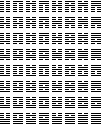
\includegraphics[scale=1]{graphics/binary-hexagrams.png}}}
    \fbox{\subfigure[Chu Hsi Hexagram Sequence]{\label{chuhsi-hexagrams}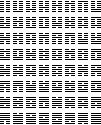
\includegraphics[scale=1]{graphics/chuhsi-hexagrams.png}}}
    \fbox{\subfigure[Gray Code Hexagram Sequence]{\label{gray-hexagrams}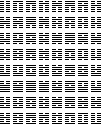
\includegraphics[scale=1]{graphics/gray-hexagrams.png}}}
	  \caption{Hexagram Sequences}
	  \label{hexagrams}
  \end{center}
\end{figure}

A more ancient permutative system is the 64 hexagrams of the I Ching. These hexagrams have been presented in a number of arrangements over time. For example: the classic King Wen sequence, The Mawangdui sequence, the Fu Xi sequence, and the Chu Hsi sequence. The King Wen sequence contains many inverted pairs but is otherwise not best understood as a mathematical system. The Mawangdui sequence is similar to concatenation of the x/y position of a hexagram when arranged in an 8x8 grid and indexed by trigrams. The Fu Xi sequence follows standard binary enumeration, and the Chu Hsi sequence follows ``De Wensput''.

I began exploring permutations not because they are a particularly effective way of revealing an embedded context, but because any enumerative piece is partially defined by which enumeration it uses. For the 64 hexagrams of the I Ching, there are $64!\approx10^{89}$ orderings---of which four are given above. For all the chords in the octave, there are $8178!\approx9.4*10^{28,463}$ possible scores. Though all of the pieces in this section use binary representations of their space, only ``The Chord Catalogue'' and ``De Wensput'' use a nonstandard enumeration.

One other permutation of binary enumeration is Gray code. Gray code has the interesting property of only changing one bit between adjacent codes. A Gray code can be enumerated recursively, or by a simple logical operation on the standard binary enumeration.\footnote{While Gray codes are a fairly recent development, they have also been used to analyze the I Ching hexagrams.\cite{Mair79}}

Unfortunately all these enumerations have two properties that make it difficult to explore a space as large as MP3. The Hamming distance\footnote{Hamming distance refers to the number of bit positions that have different values when comparing two binary codes. $0101_2$ and $1011_2$ have a Hamming distance of 3.} between nearby bit strings is very small, and the bits that are different are confined to a small region. Both of these properties are independent of bit length. This is why, out of all the pieces in this section, perhaps only ``8-bit'' and ``The Chord Catalogue'' are genuinely engaging: 256 light configurations or 8178 chord variations can be explored on a human scale. The two quietly flickering rows of ``Every Icon'' set against thirty more completely empty rows illuminates nothing more than the text paired with it: ``Given: An icon described by a 32 X 32 grid. Allowed: Any element of the grid to be colored black or white. Shown: Every icon.''
		
\section{Long Pieces}

A final technique for revealing the embedded context of a medium is examining it on an unusual scale. As examples of exceptionally long musical compositions, consider Paul Slocum's ``Pi House Generator''\cite{paul_slocum_pi_2007}, John Cage's ``Organ$^2$/ASLAP'' (As Slow As Possible)\cite{john_cage_as_????}, ``Longplayer'' by Jem Finer\cite{jem_finer_longplayer_????} and Leif Inge's ``9 Beet Stretch''\cite{leif_inge_9_2007}.

``Pi House Generator'' uses the digits of $\pi$ to generate an indefinitely long piece of house music. As $\pi$ is conjectured to be normal\footnote{A normal number contains, in every base, each digit with equivalent frequency and every finitely long combination of digits.\cite{weisstein_normal_????}}, ``Pi House Generator'' shares some characteristics with the enumerative work above, but employs repetition more literally.

ASLAP is one of the more infamous performances of a Cage piece. While the first performance lasted only 29 minutes, it is now being performed on a custom built organ at St. Burchardi church in Halberstadt, Germany. Starting with a pause in 2000, it is scheduled to last 639 years, ending in 2640.
	
Longplayer is a thousand year long composition ending in 2999. The way it solves the ``problem'' of creating a one thousand year long composition is interesting: starting with a single 20'20'' composition for Tibetan singing bowls, six two-minute segments are chosen as source material. these segments are played out of phase, and the phase slowly drifts over time. The slowest drifting phase moves with the composition, only completing its phrase when the entire composition is complete. The fastest phase makes a cycle every 3.7 days. Longplayer is regularly performed at Trinity Buoy Wharf in London, and is constantly streaming online.

``9 Beet Stretch'' takes Beethoven's ninth symphony, usually 65 to 75 minutes long, and stretches it to 24 hours with pitch correction. This is a simple act of ``slowing down''; the poetics of ``Longplayer'' without the intense compositional act.
				
\chapter{Only Everything Lasts Forever}

\section{Early Work}

My first work exploring the idea of noise as non-contextual sound was in 2007 when I developed the ``AutoLoop'' Max/MSP external\footnote{Max/MSP is an ``interactive graphical programming environment for music, audio, and media.''\cite{_products_2010}}. This system was aimed at identifying repeated sections of the audio input---self-contextualized sounds---and automatically looping them. The fact that ``repetition'' is not well defined meant that the system was never fully realized due simply to my constantly changing understanding of what constituted ``repetition''. A semi-functional version was presented at the Fall 2007 MFA show in an installation and performance. The installation consisted of two pairs of wireless microphones and headphones that allowed visitors to interact with the looping system by walking around West Hall sampling sounds. I used two pairs to emphasize the possibility that sounds may be ``repeated'' without occupying a similar space. The performance consisted of a structured improvisation on guitar in collaboration with the system, which lasted a few minutes before Max crashed.

Rather than continue exploring contextuality through looping and self-reference, I started exploring enumeration. I created an infinitely long composition called ``Every Song''\cite{kyle_mcdonald_every_2009} in 2008, which iterates through all possible songs using the equal-tempered chromatic scale. It does this as quickly as possible, with the duration of every chord determined by the lowest note in the chord, guaranteeing there is time for at least one complete cycle of every tone. It uses simple binary enumeration, and proceeds in a manner very similar to ``Every Icon'' with the exception of being infinitely long: after the first chord is enumerated, it follows with all the two-chord sequences, then three, etc.

\begin{figure}
  \begin{center}
		\subfigure[Nandhopper v1]{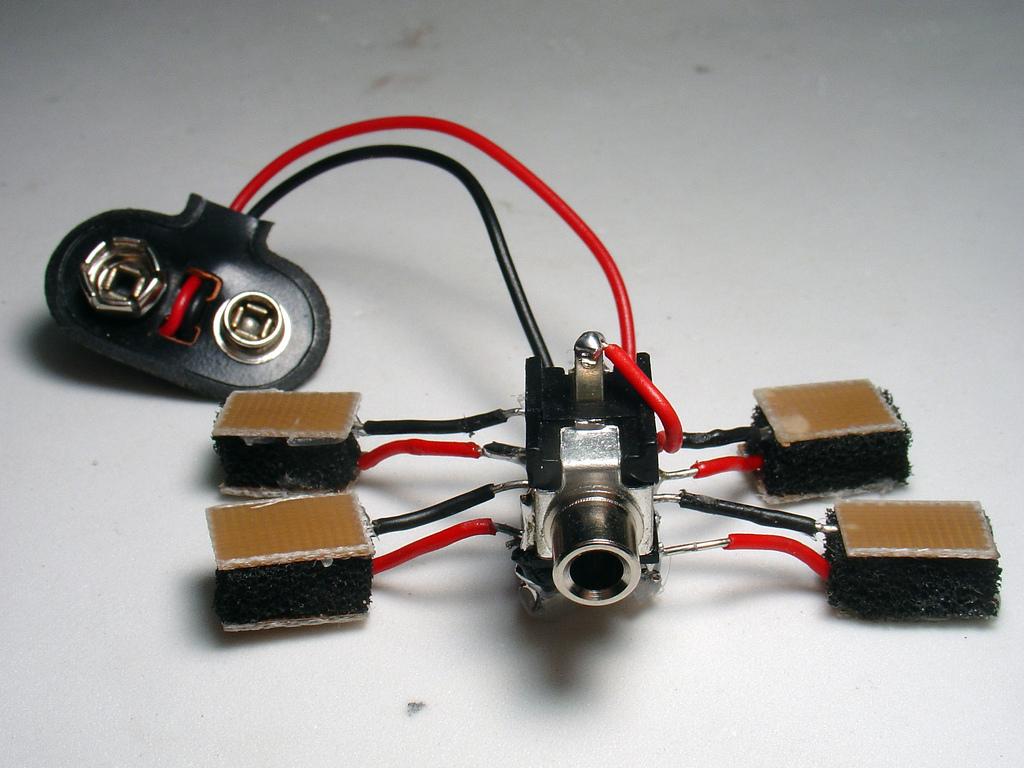
\includegraphics[scale=.2]{graphics/nandhopperv1-light.jpg}}
		\subfigure[Nandhopper v1 internals]{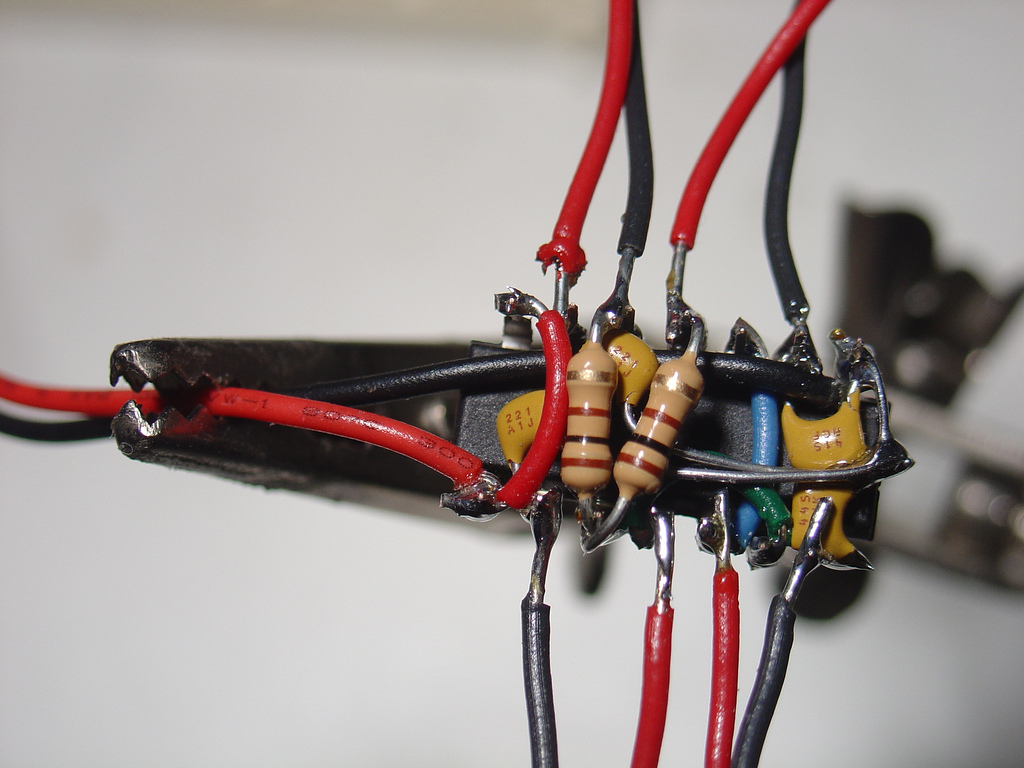
\includegraphics[scale=.2]{graphics/nandhopperv1-internals.jpg}}
    \subfigure[Nandhopper v2 off]{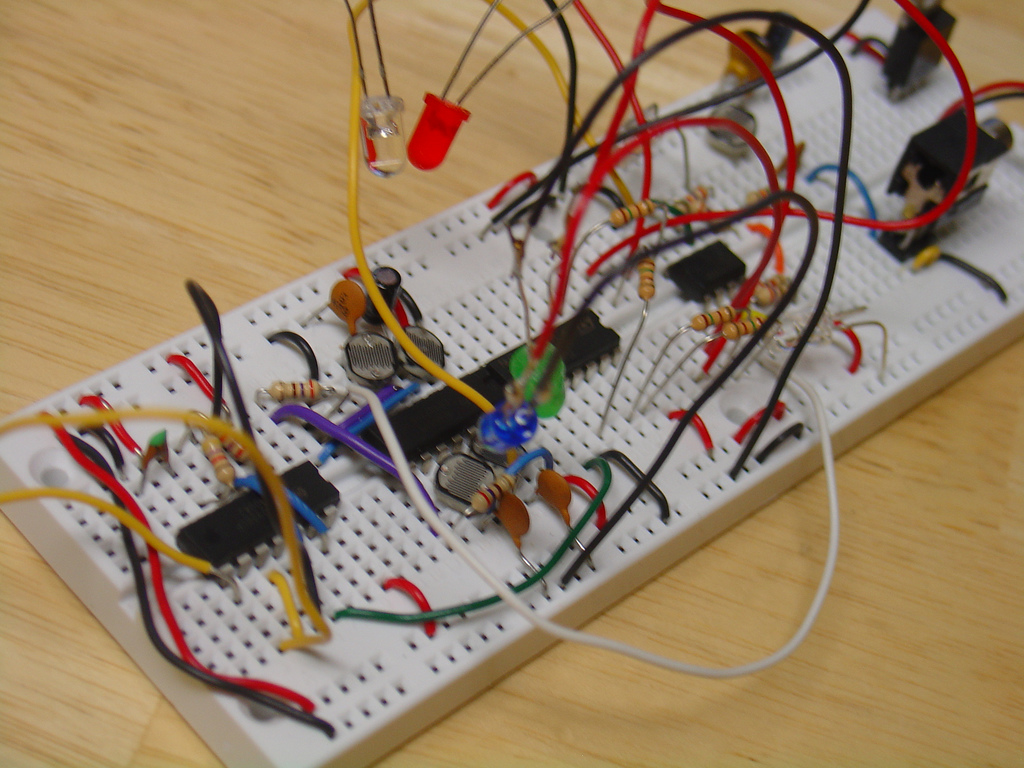
\includegraphics[scale=.2]{graphics/nandhopperv2-light.jpg}}
    \subfigure[Nandhopper v2 on]{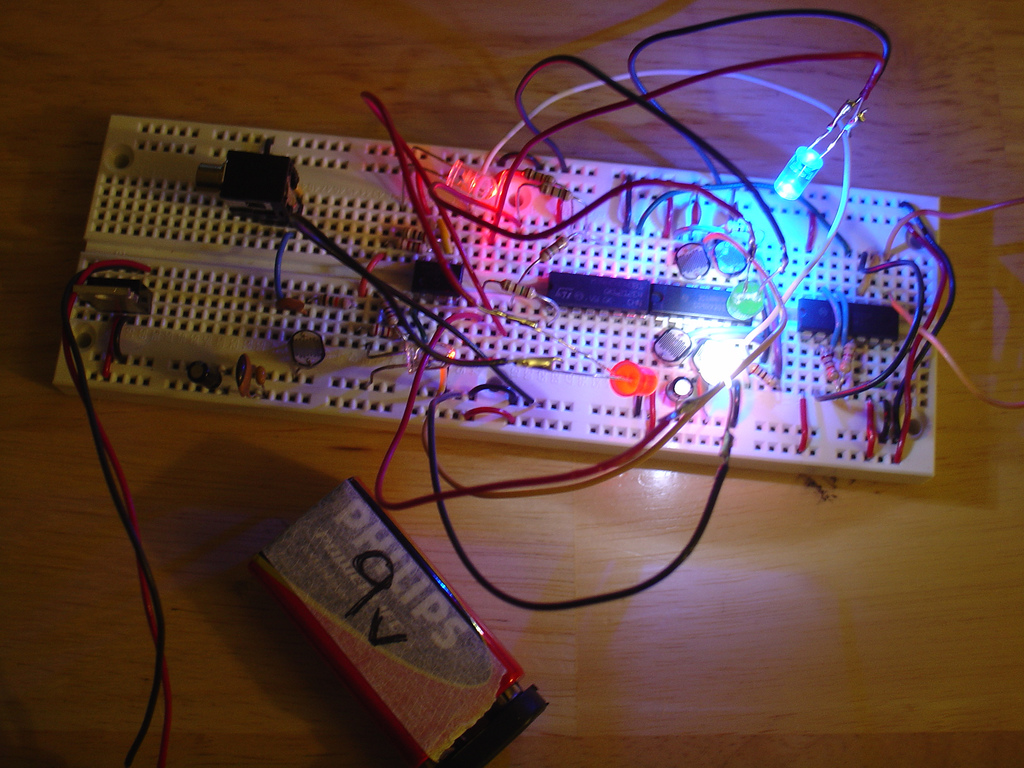
\includegraphics[scale=.2]{graphics/nandhopperv2-dark.jpg}}
	  \caption{Nandhoppers}
	  \label{nandhoppers}
  \end{center}
\end{figure}

That same summer I started my ``nandhopper'' project\cite{kyle_mcdonald_nandhopper_2008}, which also draws on enumeration. The NAND gate has the unusual property of being able to represent any possible logical operation on any number of inputs. This means that any possible digital sound synthesis circuit can be represented using only NAND gates.
	
I first came across NAND gates when exploring capacitive sensing. NAND gates are useful for constructing feedback loops that vary their frequency with respect to capacitance to ground. When I realized that NANDs could be used to simulate every other chip, I started exploring various NAND configurations and ways of connecting multiple NAND circuits.\footnote{I developed three different configurations for experimental filmmaker Diego Delmar, and later published these designs with detailed instructions on the tutorial-sharing site Instructables.com} In Spring of 2009 I developed my intuition for a complex variation on the NAND-synth for a performance environment. This variation integrated capacitive, resistive, and optical sensing in a massively entangled and environmentally sensitive feedback circuit. I see these different synthesizers as the first steps in a more general exploration of NAND-synthesis. I imagine a massive matrix of reconfigurable NAND circuits that can be rearranged during performance: constantly responding the changing flow of logic, able to simulate any imaginable digital synthesizer in a very practical sense---complex enough to be engaging, but predictable enough to be learned.

\begin{figure}
	\begin{center}
		
\includegraphics[scale=.5]{graphics/pppd.png}
		\caption{pppd}
	\end{center}
\end{figure}

This idea of ``the complete synth'' was expanded upon in 2009 with ``pppd''\cite{kyle_mcdonald_pppd_2009}, an indirect approach to enumeration via a random walk. It draws on computability theory\cite{boolos_computability_2002} and the idea of a Turing-complete system\footnote{Turing-completeness refers to the ability of a system to compute anything that can be computed.}. pppd uses a very simple esoteric programming language known as P'' (``P prime prime'') to accomplish this. While practical programming languages are full of statements like \verb!z = x + y!, \verb!println(z)!, and \verb!for(int i = 0; i < n; i++)!, P'' breaks computing down to its essentials: control flow, memory traversal, and memory manipulation---requiring only six commands. Because P'' is Turing-complete, any program you could write with a language like C++ or Java could also be accomplished with P'' (albeit in a significantly slower and heavily obfuscated manner). Because any possible program can be represented, this means that any possible digital image or sound can also be written to the program's memory space. pppd generates random valid code, and then visualizes and sonifies the memory space while running the code. In theory, not only can every image and sound be composed, but every compressed representation as well---along with the decompression algorithm. In practice, pppd produces very regular sequences of bright colors and repetitive sounds. This acts a revelation of the embedded context of P'': it is good at representing high-contrast memory sequences within small memory regions.

\begin{figure}
  \begin{center}
		\subfigure[Fragmented message]{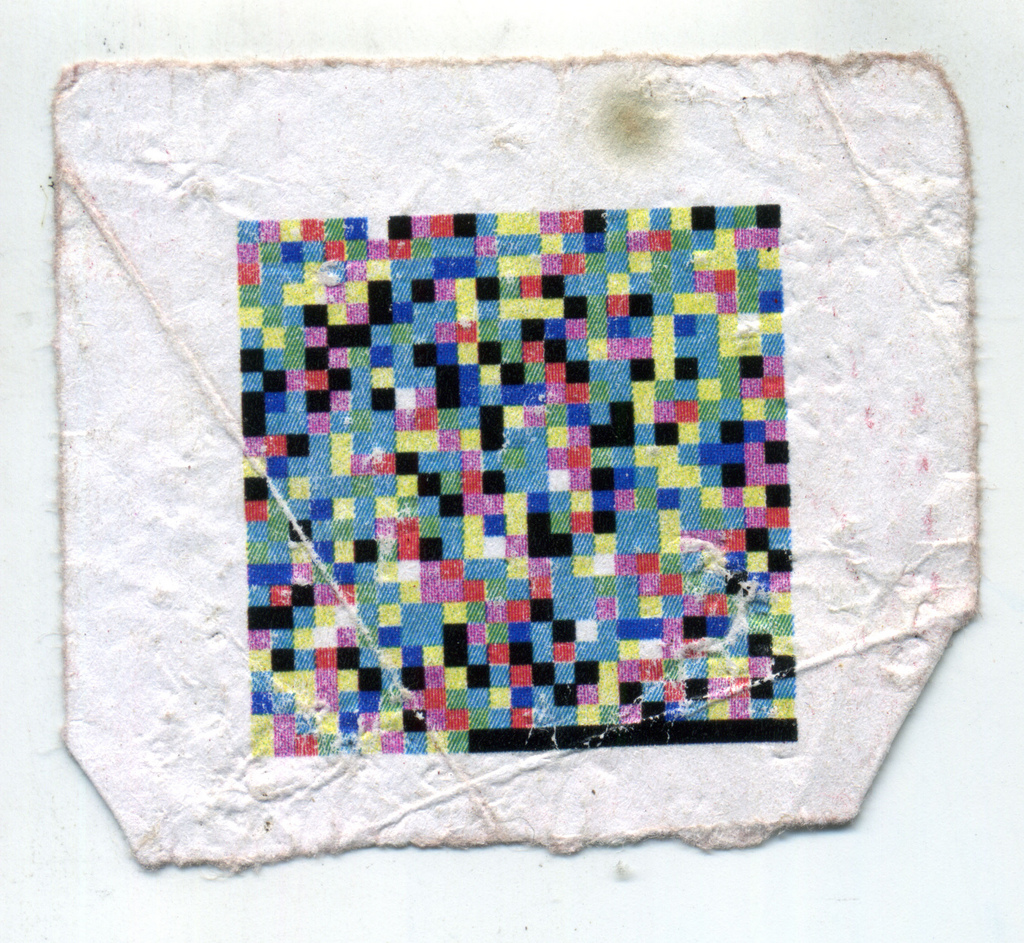
\includegraphics[height=2.5in]{graphics/futurefragments-fragment.jpg}}
		\subfigure[Decoded phonemes]{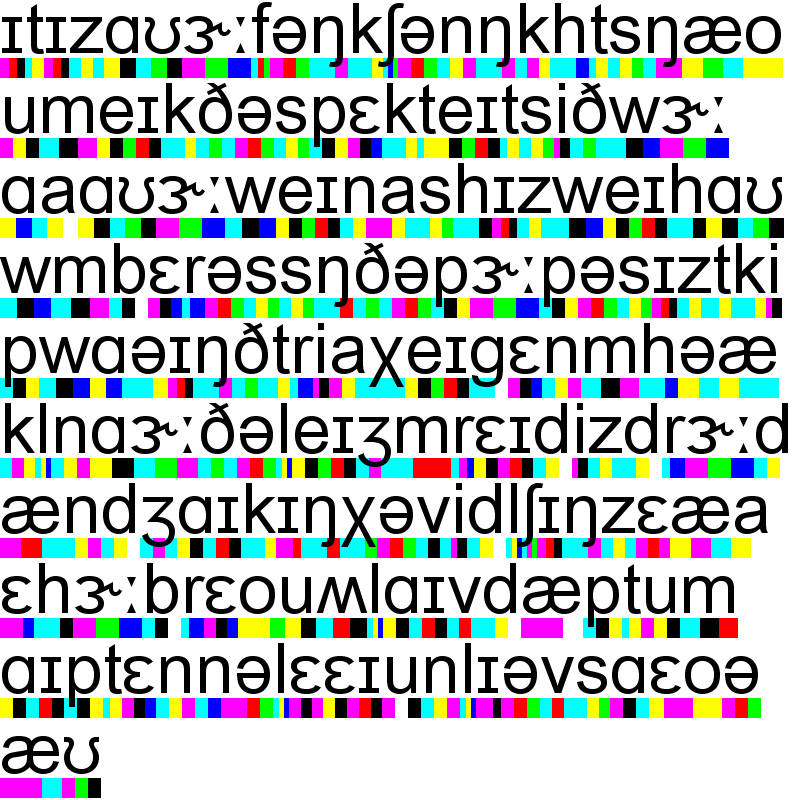
\includegraphics[height=2.5in]{graphics/futurefragments-phonemes.png}}
	  \caption{Future Fragments}
	  \label{future-fragments}
  \end{center}
\end{figure}

Also in 2009 I created ``Future Fragments''. I described it as:
	
	\begin{quote}
	An anti-time-capsule: quotes from seven fellow art students, transcribed phonetically and encoded as colors. Prints of these colors were carried by the artists for a summer. Five returned. Two extra prints were accidentally intercepted and also returned. Decoded back into phonemes and re-formed into words, each text offers an indirect account of their respective journeys.\cite{kyle_mcdonald_future_2008}
	\end{quote}

A significant portion of this piece was the time spent developing a meaningful abstract encoding for phonemes. I developed a lossless encoding that was perceptually informed so it would degrade in a perceptually relevant way.

The only other work I would self-identify as being strongly related to ``Only Everything Lasts Forever'' was a description of a piece I write in late 2009, called ``Every Every Icon'':
	
	\begin{quote}
	This work will include all of the above [two dimensional enumerative] works, as well as any other variations that may be dreamed up in the future. It will accomplish this by iterating through every possible resolution, at every possible framerate, for every possible bit depth, in every possible order.\cite{kyle_mcdonald_every_2009-1}
	\end{quote}	

\section{The History of MP3}

Another kind of context surrounding a medium might be called its ``extrinsic context'', which includes the history of its development and the various causal forces that shaped it.

While a number of researchers were involved in the various psychoacoustic and information theoretic principles underpinning the MP3 format, Karlheinz Brandenburg bears the responsibility for guiding MP3 into the form we know it today. Brandenburg's PhD advisor was interested in sending music over ISDN lines, and when the idea was rejected from the patent office for being ``impossible'' Brandenburg developed the necessary compression techniques, graduating in 1989\cite{brandenburg_interviews_2004}. The work in his dissertation went on to be further refined in collaboration with AT\&T--Bell Labs and Fraunhofer IIS, eventually becoming the ISO/IEC 11172-3, published in 1993.

MP3 takes advantage of auditory masking: our inability to distinguish weaker sonic events when they are in within temporal or tonal proximity to a stronger event or tone.\cite{Ruckert05} This might be compared to our visual system, which only detects variation in three dimensions---allowing us to represent all the varieties of spectra in their metameric three-color forms. While this perceptual coding accounts for a significant portion of an MP3's compression ratio, MP3 also takes advantage of techniques like frequency quantization and Huffmann coding.

Brandenburg admits that there are some unfortunate compromises made for MP3. Some of these are due to the fact that, as its name implies, MP3 is meant to build on its predecessors: MP1 and MP2\footnote{While Layer I is rarely used, Layer II is still sometimes used for low bitrate and speech compression applications.}. These compromises result in certain sounds, like ``dry percussive material'' (notably castanets) not translating well\cite{karlheinz_brandenburg_mp3_1999}---causing glitches like pre-echoes and bandpass filtering of higher frequencies due to MP3's limited temporal and high-frequency resolution\footnote{In a telling interview, Brandenburg actually recommends limiting the response of an MP3 encoder to 16 kHz as there ``are some hints'' that there exist listeners who can identify the difference between complex signals above 16 kHz, but ``the full scientific proof has not yet been given''.\cite[10]{karlheinz_brandenburg_mp3_1999} This bias serves as a piece of the MP3-ideology, provides the foundation for a sonic ontology, and limits musical practice as expressed within MP3.} respectively. Brandenburg himself imitates these sounds as ``shw-shw-shw'' in interviews.

While working on his dissertation, Brandenburg says he was sometimes asked ``What will happen to this?''. He would respond, ``It could end up in the libraries, like so many other theses, or it could be an international standard''. He now adds, ``I didn't dream of hundreds of millions of people''.
	
\section{The General Structure of MP3}

In order to enumerate the space of possible MP3s, it's essential to understand how the format is structured.

When I first started working with MP3, I was amazed by the way the seemingly random pattern of zeros and ones worked together to create a sound. As Brandenburg says, ``it's really a miracle with how that is reconstructed to get you the music again''\cite{tom_merritt_real_2010}. Learning the MP3 specification became a sonic practice in itself: discovering the extrinsic historical context and embedded context of a previously noisy sound.

Generating random PCM or bitmap files might be compared to placing a monkey at a typewriter: from a fixed set of symbols, they could pick any of the symbols. Generating MP3 frames is more like placing a human at the typewriter, and telling them they are allowed to type anything that conforms to basic rules of spelling and grammar. If conducted in Japanese, the resulting string of symbols would appear noisy to me apart from the superficial context of it, obviously, being Japanese---but to someone who understands Japanese there is a deep context. Likewise, the hexadecimal sequence:
	
	\begin{verbatim}
	...ff fb a2 00 ea 84 43 dc 64 56 51 ec 1d 22 7b 8c 8a ca 3d 83 a4...
	\end{verbatim}
	
Will appear noisy to the untrained eye, but to someone who understands MP3 it is obvious that this describes the header and the beginning of the side info for a stereo MP3, encoded at 160 kbps and 44.1 kHz.

An MP3 file consists of a bitstream that is divided into metadata and audio data.\footnote{Only the audio data is defined by the ISO standard, which has lead to the proliferation of metadata formats for MP3. This space has its own interesting biases. In ID3---the most common metadata format---one byte is alloted for genre, indexing a list of 148 genres. The list includes thirteen varieties of ``Rock'', from ``Southern Rock'' to ``Symphonic Rock'' and ``Gothic Rock'', without a mention of Indian classical music, gamelan, any kind of chant, klezmer, Afro-cuban music, or baroque. These kinds of biases are a necessary feature of any ontological system; a classic example being the Dewey Decimal System's bias for Christian literature.} The audio data is a sequence of logically independent frames physically embedded in two interleaved bitstreams: one stream occurs at regular intervals, the other fills the space in between. The regular data begins with an easily identifiable signature: a sequence of twelve binary ones. This sync is part of a 4 byte header that describes the high level characteristics of the current frame, such as the number of channels\footnote{MP3 includes mono and three types of stereo encoding. Any quantitative descriptions of the MP3 format given here are in reference to the mono mode, as ``Only Everything Lasts Forever'' is a mono composition.}, samplerate, bitrate, and version.
	
Following the header is 17 bytes of ``side information'' (side info). The header and side information together make up the regular bitstream, while the ``main data'' falls in between. The main data is Huffman coded,\footnote{Huffman coding is an algorithm for compressing information. It is based on the principle of replacing more commonly occurring symbol sequences with short codes, and less frequent symbol sequences with longer codes. MP3 uses a modified version of Huffman coding that allows significant variation in the length of the symbol sequences.} and the side info provides a variety of details about how to go about decoding it. Once decoded from its Huffman representation, the main data goes through a series of complex transformations informed by various settings and scalings described in the side info.

Every frame---header, side info, and main data---contains two ``granules'' that describe two consecutive chunks of audio. Sometimes granules share some of their 21 scale factors (a sort of EQ), which is why they are stored within a single frame. Each granule stores 576 ``frequency bands'', decoded into 576 PCM samples, meaning every frame consists of $2*576=1152$ PCM samples, or about 26 ms\footnote{This chunk of time is approximately in line with Bob Snyder's analysis of musical meaning and memory. 26 ms is near the boundary between ``event fusion'', ``melodic and rhythmic grouping'', which he places between 1/32 second and 1/16 second (p 12, ``Music and Memory'')} at a 44.1 kHz sample rate. To understand where these frequency bands come from, it may be easiest to explain them in terms of encoding than decoding. The 576 PCM samples for a single granule are first subdivided into 18 sections consisting of 32 samples each. Each block is then transformed into its frequency domain representation, yielding 32 frequency lines. Finally, each frequency line (an 18-element time-varying sequence) is processed using a modified discrete cosine transform that describes these time-varying sequences with respect to their regular variations.

In short, the main data stored in an MP3 is a heavily abstracted representation of the PCM data. It assumes that our understanding of sound is best represented by regularly varying frequency lines rather than as a time-varying sequence of variations in relative air pressure.\footnote{There is a lot of detail left out here involving scale factor bands, quantization, pre-emphasis, short versus long blocks, global gain, windowing, and overlap-add. All these things play a significant role in the sound of MP3, but the inverse modified discrete cosine transformation on the frequency domain representation is the heart of the algorithm.}

Late in the development of OELF I realized that the concept in its most literal sense, ``every MP3 frame'', is technically impossible to realize. Not for any reason of resources, but due to a theoretical limit. Every MP3 stream has a feature called the ``bit reservoir'' that it may use. This allows frames to be up to four kilobytes long. It relies on the fact that not every frame needs four kilobytes of data, and therefore a varying amount of space is provided depending on the psychoacoustic entropy at any moment. Unfortunately, of all the possible MP3 frames there are more long ones than short ones, meaning it is impossible to place them all in a single MP3 stream while maintaining the required average bitrate. Instead of giving up, I decided to narrow the project to all the MP3 frames with lengths less than or equal to the average bitrate---as these sounds are the most salient and evocative of the ``MP3 sound''.
	
\section{How Many Sounds Can We Hear?}

Assuming MP3 can represent all distinguishable sounds, we can approximate the number of distinguishable sounds by approximating the possible configurations of the MP3 format. If the fundamental unit of the MP3 is the frame, and we are working in mono at 64 kbit/s, every frame has an average length of 209 bytes. In mono, 17 of these bytes are dedicated to the side information and 4 are the header. Most of the variation occurs in the main data: the 188 remaining bytes. Therefore the total variation is $2^{188*8}=2^{1504}=10^{452}$. To put this in perspective, this is of equivalent complexity to performing ``The Chord Catalogue'' with not only the entire 88 keys of a piano, but also 17 additional microtonal notes between every half step.

While MP3 provides this upper bound of $10^{452}$ possible sounds, it's worth considering that Fraunhofer's more recent AAC format compresses audio twice as efficiently---halving the magnitude to $10^{226}$. Assuming the number of these ``sound-atoms'' that can be played in a year is on the order of $10^9$, playing all these sounds in succession would take $10^{217}$ years.
	
\section{Shuffle Codes}

The core of this composition is built on an algorithm I call ``shuffle codes''. The difficulty with regular enumerations is outlined in the subsection on permutation: there is no significant variation from code to code. Using a standard enumeration like binary could be compared to playing a chromatic scale: you probably wouldn't call it a ``composition''\footnote{The MP3 equivalent of a chromatic scale would be Part 4 of the ISO/IEC 11172-3 standard, which provides a set of MP3 files that must be decoded to within a certain RMS error of a reference decoding. Every compliant MP3 decoder has had to process this set of files at some point.}, but you might use that label for Schoenberg's 12-tone work.

Shuffle codes allowed me to maintain the spirit of enumeration behind the composition while providing plenty of parameters to tweak and distribute over the sonic space.

Organizing a huge space like that of MP3 frames might be compared to constructing a tessellation. You begin with a simple shape already known to tessellate, and then modify it by removing sections from one side and adding them to the opposite side. Because the total area of the shape is maintained, and every edge always fits into its opposite, you are left with a new tessellating shape.

Likewise, with an enumeration you must begin with an algorithm known to enumerate the entire space. Chu Hsi's arrangement of the hexagrams, Johnson's ``The Chord Catalogue'', standard binary enumeration, and Gray codes all fulfill this requirement. From there you can apply a one-to-one function over the enumerated codes that reorganizes or remaps them. One-to-one functions guarantee that no two codes are mapped to the same code---thereby preserving the property of complete enumeration. An example of a one-to-one function would be digit reversal---mapping 7,419 to 9,147\footnote{One way of knowing this is a one-to-one function is that a simple algorithm exists for transforming it back into the original value. In the case of digit reversal, the algorithm simply needs to be applied again.}.

\begin{figure}
	\begin{center}
		
\includegraphics[scale=1.5]{graphics/gray-operation.pdf}
		\caption{Gray Code operation}
		\label{gray-operation}
	\end{center}
\end{figure}

Shuffle codes are constructed using the iterative application of two one-to-one functions. The first is the standard Gray code operation, consisting of a single bit shift followed by an XOR against the original value as shown in Figure~\ref{gray-operation}. The Gray code operation has the helpful property of spreading bits out.

The second operation is the digit shuffle. Digit shuffling consists of reordering the digits of a number. Digit reversal is one kind of shuffling technique, one of $n!$ possible techniques for a set of numbers with $n$ digits. If the shuffling technique has both local and global movement---ensuring that two adjacent digits do not necessarily remain adjacent after being shuffled---then a pseudorandom chaotic behavior emerges from the iterative application of the Gray code and digit shuffling.

\section{Composition as Bit Placement}

This pseudorandom behavior can be controlled by crafting alternative shuffling techniques. The first shuffling technique I used was based on digit reversal, but this did not fulfill the global movement requirement and lead to a very low variation between codes. Next I implemented a shuffling technique that moved digits to a new position based on a bitwise reversal of their original position\footnote{For example, in a code with length 32, the digit at position $26_{10}=11010_2$ would be moved to $11_{10}=01011_2$}, as shown in Figure~\ref{reversal-shuffle}.

\begin{figure}
	\begin{center}
		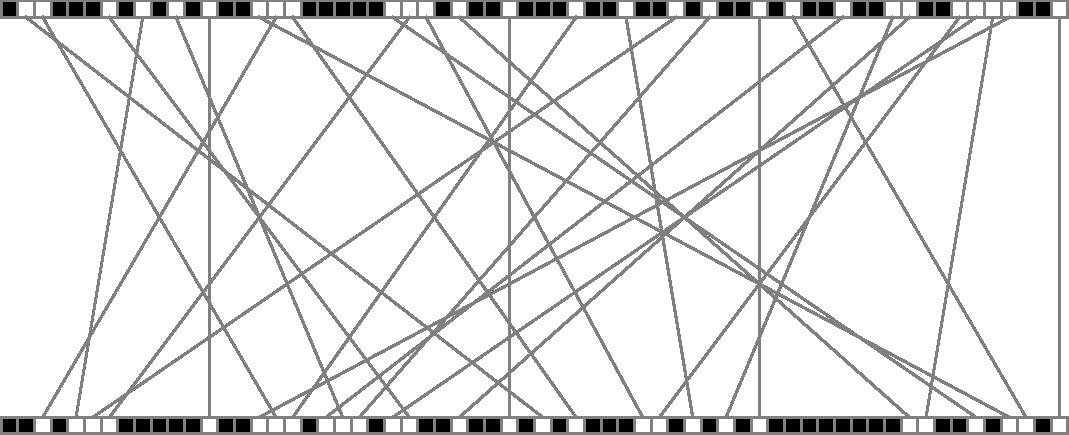
\includegraphics[scale=.5]{graphics/reversal-shuffle.pdf}
		\caption{Digit reversal shuffle example}
		\label{reversal-shuffle}
	\end{center}
\end{figure}

This lead to an enumeration that was uniformly pseudorandom across all the bits, as shown for the 16-bit case in Figure~\ref{enumeration-diagram}. While this variation is exactly what I was originally looking for, I soon realized that I was left with almost no lower frequency variation to compose with. After manual tweaking of the shuffling technique, I settled on a swap-based shuffle that slowly progressed from local movement to global movement over the length of the digits, shown in Figure~\ref{swap-shuffle}. This provided both low frequency variation on the order of days and weeks up to high frequency variation on the order of a single frame.

\begin{figure}
	\begin{center}
		
\includegraphics[scale=.5, angle=90]{graphics/enumeration-diagram.pdf}
		\caption{Digit reversal shuffle code derivation}
		\label{enumeration-diagram}
	\end{center}
\end{figure}

\begin{figure}
	\begin{center}
		
\includegraphics[scale=.5]{graphics/actual-arcs.pdf}
		\caption{Swap-based shuffle technique}
		\label{swap-shuffle}
	\end{center}
\end{figure}

With the enumeration developed, it was then placed in an MP3 ``skeleton''. I decided to use a 64 kbp/s at 44.1 kHz mono format, as I see 128 kbit/s at 44.1 kHz stereo as the quintessential MP3, but wanted to use a mono signal. There are also two curious bits in the MP3 header that required a decision: the ``copyright'' and ``original'' bits. These were originally meant to indicate whether a file was copyrighted and, if not, whether it was a copy. In ``Only Everything Lasts Forever'', both of these bits are set to false. Some bits within the side info were also set in order to limit the maximum frame length and avoid the technical limitation mentioned at the end of the section ``The General Structure of MP3''.

The final steps involved lots of listening; tweaking the shuffle technique and the final placement of the bits in the resulting enumeration. The bit placement was informed by an earlier composition for MP3 presented at the Spring 2009 MFA show. This composition was essentially a glitched recording of 4'33'' broadcast by BBC Radio 3 in 2004\cite{_radio_2004}. The glitches were introduced by parsing an MP3 of the recording, modifying logically distinct portions of the bitstream, and writing out the modified version. I developed a basic glitch sequencer that allowed me to craft the glitches over time, translating a graphic score from my sketchbook into a series of bitwise manipulations. The score was preceded by experiments with ``linear'' MP3 glitching where I would modify one parameter at a time---for example, using a fixed value for the global gain, which causes dynamic range compression. I only explored variation in the side info, as it took another half year to completely understand the main data. For ``Only Everything Lasts Forever'', I used the technical knowledge and intuition gained from these experiments to help me place bits of different variation in the MP3 frame---for example, placing the bits with more variation in the higher frequency end of the main data, and using bits with lower frequency variation for more global features in the side info like Huffman table selection and scale factor bands (introducing some rhythmic regularity). Moving from this earlier composition to ``Only Everything Lasts Forever'' also required a complete rewrite of the analysis and MP3 synthesis code, from Java to C++, as the Java was difficult to optimize for real time streaming.

\section{Presentation}

The premiere of ``Only Everything Lasts Forever'', an excerpt of the first month streamed over the Internet, began on March 28th, 2010 at 7PM EST\footnote{The stream went live an hour before the composition began, and during that time I streamed live audio from the hum of the server room using the laptop's built in microphone.}. The idea of using an internet stream was inspired by projects like ``Eigenradio'', ``Longplayer'', and ``9 Beet Stretch''.

The server broadcasting the stream---an old laptop on loan from a friend---was installed in a server room on the seventh floor of the Experimental Media and Performing Arts Center (EMPAC) on the Rensselaer Polytechnic Institute campus. Every hour, on the half hour, the next hour of the composition is generated and added to a Winamp playlist\footnote{Winamp is a ``media player that plays mp3 + other audio files''\cite{_winamp_????}.}. It takes about half a minute to generate each hour of music. Winamp then streams to a Shoutcast\footnote{Shoutcast is comprised of software that can be used for webcasting MP3 and AAC audio streams as well as a website indexing these webcasts\cite{_shoutcast_????}.} server on the same machine, relaying the stream to listeners. While MP3 files are generally decoded and re-encoded into a consistent format for internet radio streams, my original intention was to stream the generated MP3 without decoding it---meaning that the signal would only exist in the time domain when decoded on a listener's computer. In the end, I had to re-encode the generated MP3s due to compatibility issues\footnote{When sharing early iterations of the project, the same MP3 would be decoded differently depending on the decoder. One friend even reported that listening to the MP3 caused his sound card to crash, and forced him to restart his computer.}.

Two days after the stream began, on Tuesday March 30th, I held a reception that was aimed primarily at encouraging discussion and secondarily at providing a listening environment. My laptop stood on a pedestal in the center of the room with closed ear headphones plugged in, displaying a simple visualization of the MP3 frame generator and streaming the live audio from the server at EMPAC. Two low tables in the room held a number of books referenced in this paper and the three sketchbooks I've used while developing this piece. Each book contained at least one post-it note describing the connection between the book and ``Only Everything Lasts Forever''. I tried to create a space for informal discussion by informing people that I would speak briefly half an hour into the opening, which allowed people to comfortably talk to each other for half an hour while waiting. After giving an explanation of the motivation for and content of the piece, I held a longer-than-expected question and answer session.

Over the course of the first month, the stream has had about 180 unique listeners at 320 different times, with a mean listening time of 18 minutes and mode of 1'33''. Over half of the listens happened in the first three days, with only a handful of listeners regularly returning throughout the month.

Further documentation and excerpts are available on my website\cite{kyle_mcdonald_only_2010} and as a publicly accessible open source project\cite{kyle_mcdonald_oelf_2010}.

\chapter{Conclusion and Future Work}

``Only Everything Lasts Forever'' started as an exploration into enumerating the space of our psychoacoustic awareness, and evolved into an attempt at revealing the embedded context of the MP3 format. I wanted to make a sound work that was more interesting to listen to than ``Every Icon'' is to watch. I challenged my own understanding of what constitutes noise and non-noise, and explored my definition of noise as non-contextual sound.

I feel like ``Only Everything Lasts Forever'' succeeds in that it enumerates the space in an interesting way, and provides a good sense of the inherent biases of MP3. On the other hand, I feel like it fails whenever I spend more time talking with someone about it than they spend listening to it. The protagonist of Borges' ``The Aleph'' makes an interesting comment about the difference between how a work is received and how it is justified:
	
	\begin{quote}
	[...] Daneri's real work lay not in the poetry but in his invention of reasons why the poetry should be admired. Of course, this second phase of his effort modified the writing in his eyes, though not in the eyes of others.
	\end{quote}
	
Perhaps this distinction between affective power and conceptual admiration emerging from reflection is also what John F. Simon Jr. was referring to when he wrote:
	
	\begin{quote}
	While Every Icon is resolved conceptually, it is unresolvable in practice. In some ways the theoretical possibilities outdistance the time scales of both evolution and imagination.\cite{john_f._simon_jr._given:32_1997}
	\end{quote}

While Yasunao Tone may not be for everyone, some of his ideas are made significantly more accessible by ``Oceanic glitch''\cite{Sangild04} artists like Oval and Oto---you don't need to know CD glitching is involved to appreciate their work. I would like to continue working with MP3 in a way that is more accessible, without forfeiting any conceptual depth. Each sound in ``Only Everything Lasts Forever'' is contextual in that it is derived from the causal web that lead to the composition, including the embedded and extrinsic historical contexts of the MP3 format and its psychoacoustic foundation. But there is a deeper context to accessible sounds based on the sonic intuition of the composer. I think the primary difficulty of working with an enumerative composition is that the constraint of total enumeration requires composition to occur at a highly abstracted level, leaving little room to integrate that sonic intuition.

There are three directions I would like to take this work. First, simply removing the constraint of total enumeration, opening up the possibility of a work with more locally composed variation. For example, simply changing the digit shuffling technique has a huge effect on the sound of the composition, but it's not possible to change the technique over the course of the composition without breaking the enumeration constraint. Second, I would like to work with found MP3s---reorganizing frames from unheard songs in stockpiled music libraries, or combining frames to create Frankenstein sounds where one frame describes the format while another provides the content. Third, I would like to extend these techniques to instruments and effects. For example, a VST plugin that encodes audio into MP3 frames and decodes back into PCM on the fly, allowing the user to glitch portions of the frame in real time, providing a much more direct method of MP3-collaboration than the slow, unwieldy cycle of coding and compilation.

Other directions include alternative methods for presenting the composition. Drawing on ``The Aleph'' again, using a speaker hidden behind an otherwise featureless wall in some public space. This may provide the most fitting environment for this composition, allowing visitors to pass by, aware without listening; or listening regularly but momentarily---like the title, offering a gentle reminder in the face of our most common misunderstanding.

\specialhead{Bibiliography}
\begin{singlespace}
%\bibliographystyle{plain} % alphabetical
\bibliographystyle{unsrt} % in order of appearance
%\bibliographystyle{mla-good} % mla
\bibliography{original,zotero}
\end{singlespace}

\end{document}
